\section*{Lezione 16}
\addcontentsline{toc}{section}{Lezione 16}

\subsubsection*{Crittosistema Playfair '800}

Esso è un crittosistema polialfabetico che cifra a coppie. La chiave è formata da un quadrato di $5 \times 5$ lettere inglese (tranne la \texttt{J}). Sì, c'è solo una chiave.
Il testo in chiaro $m$ è splittato in blocchi di due lettere (questi blocchi non possono contenere doppie)
\begin{itemize}
	\item \textbf{Cifratura:} ogni blocco è crittato separatamente:
	\begin{itemize}
		\item Se due lettere sono sulla stessa riga allora ci si sposta ciclicamente verso la destra (ogni lettera diventa la sua adiacente a destra)
		\item Se due lettere sono sulla stessa colonna allora ci si sposta verso il basso
		\item Altrimenti esse individuano un rettangolo, quindi prendo gli altri due vertici del rettangolo
	\end{itemize}
\item \textbf{Decifratura:} si fa lo stesso procedimento però all'inverso
\end{itemize}
Per creare una chiave si parte da una frase:
\begin{center}
	\texttt{COURSE ON CRYPTOGRAPHY}
\end{center}
si rimuovono le lettere che occorrono più volte:
\begin{center}
	\texttt{COURSENYPTGAH}
\end{center}
poi completiamo inserendo le altre lettere:
\begin{center}
	\texttt{COURSENYPTGAHBDFIKLMQVWXZ}
\end{center}

\'E facile da ricordare e da ricostrutire, però è facile da indovinare (la prima parte è una parola, le ultime sono le rimanenti dell'alfabeto).
Dal punto di vista della crittoanalisi: ogni paio di lettere individua sempre lo stesso blocco (si possono fare analisi delle frequente ecc.).

\newpage

\subsubsection*{Crittosistema Vigenère '500}

Funziona come il cifrario di Cesare, però la chiave cambia dopo aver cifrato ogni lettera.
La chiave è composta da una parola, ripetuta più volte fino ad arrivare alla lunghezza del testo in chiaro $m$.

\begin{figure}[h]
	\centering
	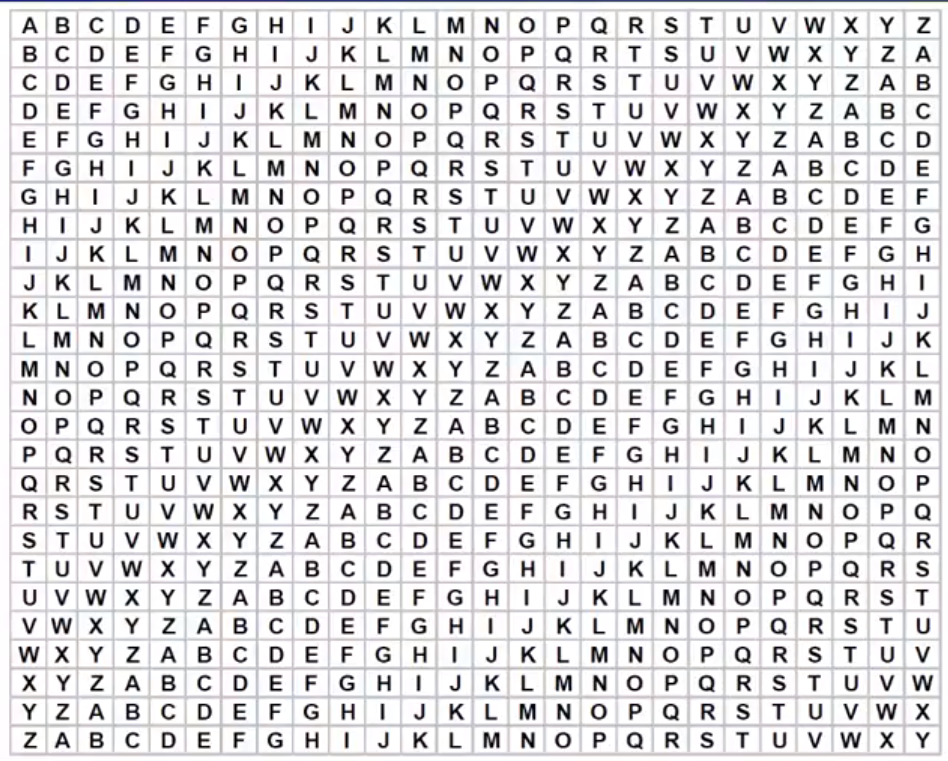
\includegraphics[width=0.8\linewidth]{immagini/img33}
\end{figure}

\begin{itemize}
	\item \textbf{Cifratura}: ogni paio di lettere di $m$ e $k$ individua una riga e una colonna, si prende il carattere che è contenuto nella cella a cui si riferiscono.
	Esempio: $m$: \texttt{PURPLE}, $k$: \texttt{CRYPTO}, $c$: \texttt{RLPEES}.
	Ad esempio il primo carattere sarà quello individuato dalla riga che inizia per \texttt{P} e la colonna che inizia con \texttt{C}.
	\item \textbf{Decifratura}: le stesse operazioni all'inverso.
	\item \textbf{Crittoanalisi}: la i-esima lettera di $m$ è cifrata come Cesare, la cui chiave è la i-esima lettera della chiave. Se la lunghezza della chiave è $l$, allora le lettere di $m$ in posizione $i$, $i+l$, $i+2l$... sono tutte cifrate con la stessa lettera di $k$.
	Ad esempio per $l = 5$, scrivo i caratteri del testo cifrato in righe lunghe $l$, quindi avrò (in termini di posizioni):
	\begin{equation*}
	\begin{matrix}
	1 & 2 & 3 & 4 & 5\\
	6 & 7 & 8 & 9 & 10\\
	11 & 12 & 13 & 14 & 15\\
	\vdots & \vdots & \vdots & \vdots & \vdots
	\end{matrix}
	\end{equation*}
	A questo punto ogni colonna è cifrata con la stessa chiave di Cesare, per cui si può effettuare un'analisi delle frequenze.
	Questo rompe il sistema anche se il numero delle chiavi è $26^5 = 11.881.376$.
	Come si trova però la lunghezza della chiave? Cerchiamo delle occorrenze di alcune sequenze, \texttt{PUXUL} + 15 lettere + \texttt{PUXUL}. La lunghezza della chiave potrebbe essere un divisore di 20.
	min 35 p1
\end{itemize}



